\chapter{Background}

Understanding Jester's core functionality requires background knowledge of how 3D positions can be transformed into different coordinate spaces and how quaternions handle rotations. The peripheral technologies like ranging solutions and filtering algorithms also warrant explanation. These technologies will be briefly explained in the following subsections.

\section{Spatial Mathematics}

Jester stores its skeletal representation as a hierarchy of bones where each bone stores its position and orientation relative to its parent bone's coordinate space. It also provides the ability to set bone positions from skeletal joint coordinates in arbitrary space. The design and implementation of the bone hierarchy and joint transforms will be discussed in Section \ref{sec:bone_hierarchy}. Understanding the bone hierarchy and joint transforms will require a basic understanding of matrix spatial transforms and quaternions.

\subsection{Spatial Transforms}

3D objects are defined within a coordinate space. In the Cartesian style spaces used in Jester, each dimension of the space is specified by a 3D vector, or basis vector, that is defined in its parent space \cite{gortler2012foundations}. All of Jester's basis vectors are orthonormal, meaning they are orthogonal and unit length. Orthonormal bases simplify the process of reasoning about skeletal positioning because they guarantee that all of the dimensions can be measured with the same units. Spaces do not have to be specified in this manner, but more complex spaces are unnecessary for this application and lie outside the scope of this thesis. 

\begin{figure}[h]
\centering
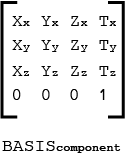
\includegraphics[width=0.25\textwidth]{figures/transMatrix}
\caption{Transformation matrix components.}
\label{fig:transformation_mat}
\end{figure}


Jester spaces are specified in the traditional 3D computer graphics style where a 4x4 matrix, also known as a transformation matrix, is used to define and represent the space. The transformation matrix is constructed by combining the x, y, and z basis vectors with a vector specifying the translation of the new space within its parent. The 4th row of the matrix holds a basis vector that allows the matrix to be used for affine transformation. The layout of the matrix is shown in \ref{fig:transformation_mat}. A 3D point specified in the new space can be converted, or transformed, into the corresponding 3D point in the parent space by multiplying the point by the transformation matrix of the new space. In order for the multiplication to be possible, a fourth dimension must be added to the point. The fourth dimension is known as the homogeneous component and allows points and vectors to be handled correctly \cite{roberts1963machine}. Similarly, a 3D point can be transformed from the parent space to the child space by multiplying the point by the inverse of the child's transformation matrix.

\subsection{Quaternions}

Quaternions are a complex mathematical construct that effectively store a 3D axis and the amount of rotation around that axis. They are less intuitive than Eulerian rotations, which are a combination of three rotations about the x, y, and z axes, however, they allow for rotations to be combined without the possibility of Gimabl lock. Gimbal lock occurs when rotation about one axis causes the other two axes to be on the same plane. If two axes are coplanar a degree of freedom has essentially been lost \cite{gortler2012foundations}. Figure \ref{fig:gimbal_lock} demonstrates how a 90 degree rotation about the red axis causes the green and blue axes to both specify rotation about the same axis.

\begin{figure}[h]
\centering
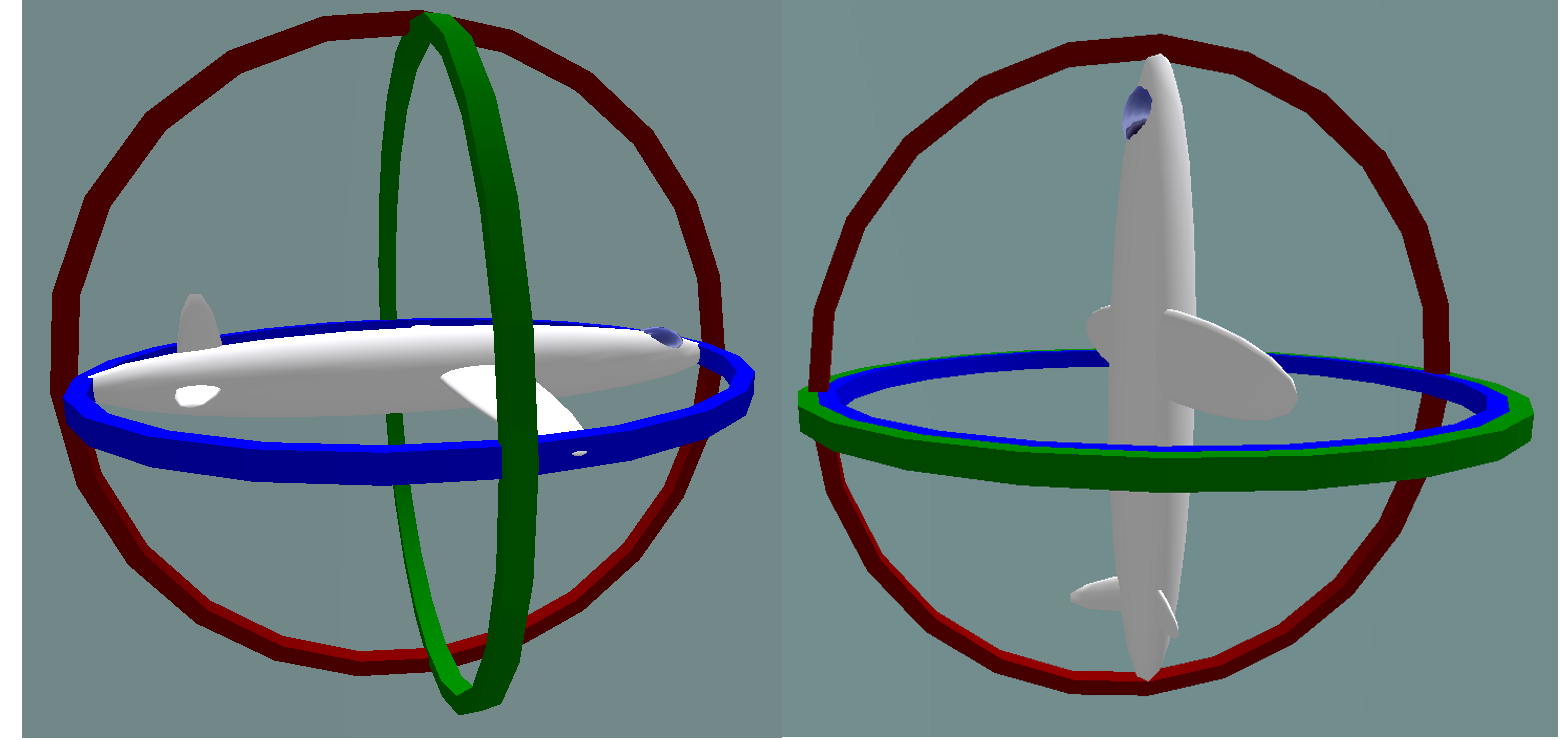
\includegraphics[width=0.75\textwidth]{figures/gimbals}
\caption{Gimbal lock when two axes are rotated onto the same plane. Credit: ``MathsPoetry" (Wikipedia Commons)}
\label{fig:gimbal_lock}
\end{figure}

\section{Sensor Types}

There are many different sensors that have begun to become popular in the consumer 3D input device market. They can be broadly broken into two categories: devices that require the user to wear trackable markers or sensors, and devices that use some form of imaging technology to observe the scene. Both categories contain many sub-types. Some current commercial examples will be examined and broadly explained. Jester is capable of working with any sensor that can produce data about a joint's or bone's position and orientation. The process of using the sensor with Jester will be explained briefly below. More detail about the Jester API and its use can be found in Section \ref{sec:sensor_wrappers}. 

\subsection{Wearable Sensors}\label{sec:wearables}

Wearable sensors require that either trackable objects or the actual sensor itself is placed on the body part that the user wishes to track. They have the advantage of being very resistant to interference from ambient light, and are generally more accurate than other approaches. The trade off is that there is more setup time involved to place sensors and each bone or joint requires a separate sensor or marker \cite{zhu2004real}. Figure \ref{fig:wearables} shows the wearable sensors that will be discussed in the following sections.

\begin{figure}[h]
\centering
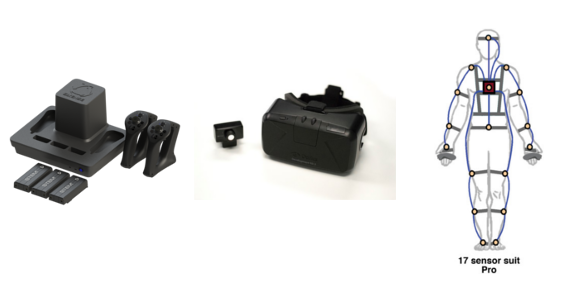
\includegraphics[width=1\textwidth]{figures/wearables}
\caption{Wearable sensors. Left to Right: Sixense STEM, Oculus Rift, PrioVR Suit. Source: Press Materials \cite{sixense_stem, oculus2012oculus, priovr}}
\label{fig:wearables}
\end{figure}

\subsubsection{Sixense STEM}\label{sec:sixense}

One example of a wearable sensor is the Sixense STEM. The Sixense STEM system can track up to 3 remote tags, STEM packs, and two handheld controllers in the x, y, and z dimensions as well as the roll, pitch, and yaw, known as six degrees of freedom, using magnetic field sensors (6 DOF) \cite{sixense_stem}. Relying on magnetic field rather than some sort of visual sensor means that the STEM system is impervious to any sort of lighting or UV interference. Using the STEM system with Jester would be as simple as getting the controller and STEM pack data from the Sixense API, associating the data points with the correct Jester bones or joints, and calling the newData() function on the Jester Controller.

\subsubsection{Oculus Rift}\label{sec:oculus}

The Oculus Rift is primarily a head mounted display, but it accurately detects head orientation using gyroscopes in order to provide the ability to look around the virtual environment \cite{oculus2012oculus}. The orientation returned by the Oculus API could easily be assigned to the head bone and then fused with the head position given by some other sensor in the Jester data fusion framework to provide both head orientation and position with minimal overhead.

\subsubsection{PrioVR}\label{sec:prio}

Yeti Technology is set to start delivering the first units of its new PrioVR system in Fall of 2014. The PrioVR system provides a set of Inertial Measurement (IMU) sensors that are designed to be attached to all of the main extremities on the user. The sensors reconcile their positions against the position of the main sensor unit which is mounted near the sternum to establish the pose of the user \cite{priovr}. PrioVR is perfectly suited to send data to Jester since it already senses the position and orientation of all of the major bones that are tracked by Jester.

\subsection{Imaging Sensors}

Imaging sensors capture the light reflected off of the user in order to determine his position. Some emit their own light in order to simplify the process of ranging and others rely entirely on ambient light. Therefore, all of them are sensitive to ambient lighting conditions and can be rendered ineffective by either too much ambient light or, in the case of passive sensors, not enough \cite{besl1988active}. They do not require markers to be placed on the user and can be designed to have very minimal setup times. Some examples of imaging sensors and their consumer implementations are discussed below.

\subsubsection{2D Cameras}

Traditional 2D cameras can be used to gather skeletal data. Extensive research has been done in attempting to subtract irrelevant background from 2D images and isolate the desired features. However 2D imaging techniques remain very sensitive to differences in ambient light and background color or texture. Due to these limitations, 2D cameras are not frequently used in consumer 3D user input devices that expect a reasonable level of accuracy \cite{shimada2001real}.

\subsubsection{Structured Light}

Structured light sensors work by emitting a pattern of infrared light like the one shown in Figure \ref{fig:carmine_light}. When the pattern strikes objects, it is distorted based on the angle of the object and its distance to the sensor. The sensor has a camera that is designed to only respond to infrared light that captures how the emitted pattern is reflected off of the user. The sensor then internally maps the emitted pattern to the distorted pattern to figure out pattern's transform. The transform gives the distance to that particular part of the image. The sensor combines all of the distances into a depth image where grayscale color corresponds to the distance to that particular pixel. If any ambient light source produces more infrared light than the emitter, structured light sensors lose accuracy very quickly \cite{scharstein2003high}.

\begin{figure}[]
\centering
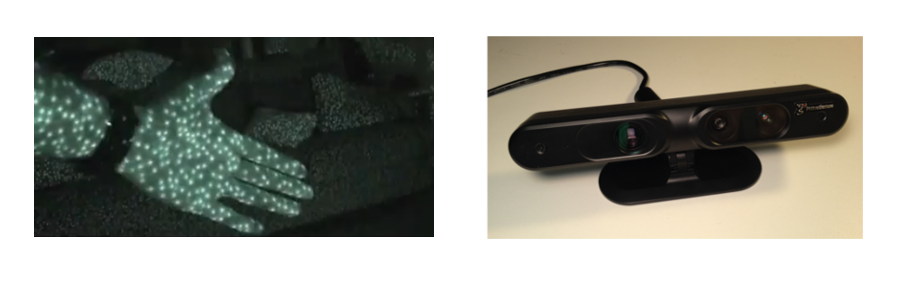
\includegraphics[width=1\textwidth]{figures/carminePattern}
\caption{PrimeSense Carmine and the structured light pattern it emits. Source: \cite{structured_pattern}}
\label{fig:carmine_light}
\end{figure}

The PrimeSense Carmine and the Kinect are both examples of structured light sensors. They have an effective range of approximately 1 to 3 meters and have supporting libraries that map the output depth image to an estimated model of the user's joint positions. These joint positions can be fed directly into Jester and Jester will reconstruct the position of the skeletal bones using known mappings from joints to bones. The Jester example program presented in this thesis uses the PrimeSense Carmine and will be discussed in more detail in Section \ref{sec:carmine_impl}.

\subsubsection{Time of Flight}

Time of flight sensors, at a high level, emit pulses of light and then measure how long the light takes to return to the sensor in order to estimate distance. They are much more accurate than structured light sensors and are less sensitive to ambient light because they are not attempting to interpret a pattern of light, just the existence of return pulses \cite{litime} Figure \ref{fig:tof} explains the ranging technique used in the Texas Instruments time of flight sensor. 

\begin{figure}[]
\centering
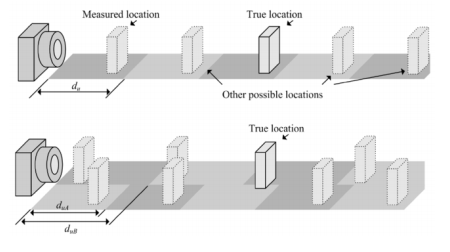
\includegraphics[width=0.5\textwidth]{figures/tilight}
\caption{The Texas Instruments TOF sensor uses different pulse frequencies to disambiguate range. Source: \cite{litime}}
\label{fig:tof}
\end{figure}

Time of flight is replacing structured light as the technology of choice for many depth cameras. Microsoft has switched to time of flight technology for the second version of the Kinect \cite{kinect2}. Intel has partnered with Creative to subsidize the Senz3D sensor in order to push gesture-based interaction more into the mainstream. Both the manufacturer of the camera, SoftKinetic, and Intel have APIs for the Senz3D that track fingers on a hand \cite{senz3d}. The finger tracking data can be attached to the Jester hand bones and sent into the Jester API.

\subsubsection{Stereo Cameras}

Stereo camera systems are, at their simplest level, two of the same model of camera mounted a known distance apart from each other. Depth can be estimated by capturing an image from both cameras simultaneously, finding the common elements in both images, and calculating the distance based on the known distance between the cameras and the difference in position of the common elements in the images. Generally speaking, a smaller difference means the objects are far away from the camera and a larger difference means that they are closer \cite{lucas1981iterative}. Stereo cameras can either rely on natural light, or be assisted by infrared LEDs. Assisted stereo cameras are more impervious to varying lighting conditions, so the stereo setups in the commercial market are generally assisted.

One well known assisted stereo camera is the LeapMotion Controller shown in Figure \ref{fig:leap}. The LeapMotion Controller uses two cameras augmented with three infrared LEDs and is placed on a desktop facing upwards at a user's hands. It resolves the distance to the hands and attempts to pick out the user's individual fingers \cite{weichert2013analysis}. The LeapMotion Controller has an API that can be queried for hand and finger position. The Jester usage example presented in this paper uses the Leap API and will be discussed in greater detail in Section \ref{sec:leap_impl}.

\begin{figure}[]
\centering
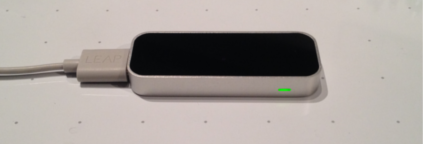
\includegraphics[width=0.5\textwidth]{figures/leap}
\caption{The LeapMotion Controller on a 1" dot grid for scale.}
\label{fig:leap}
\end{figure}

\section{Filtering Algorithms}\label{sec:filter_back}

Positional data that comes from any real world sensor is subject to some level of noise and inaccuracy. Filtering algorithms attempt to establish some sort of likelihood model for new sensor readings in order to ``trust" good measurements more than bad measurements. This is particularly useful for skeletal tracking sensors because tracking errors can sometimes occur that cause the estimated position of bones to jump wildly and then return to a consistent track. Good filtering algorithms will not assign much weight to the jumping measurements and so the filtered skeleton will be much more stable. Two filters that are well documented and have a strong following are Kalman filters, and double exponential filters. Jester supports filtering plugins and an example double exponential filter has been implemented.

\subsection{Kalman Filter}

The Kalman filter was introduced by Rudolf Kalman in 1960 as a new solution to linear filtering and prediction. His filter observes how measurements of a linear system change over time and attempts to estimate the true state of the system. Kalman filters operate using an update loop that for each iteration takes the current state of the system, uses a linear estimator function to guess how the system will change between measurements, corrects the estimation using the next sensor measurement, and sets the current system state to the corrected estimation \cite{kalman1960new}. 

The closer that the measurement is to the estimated state the more effect it will have on the system state. Measurement error is assumed to be Gaussian, which means that readings should be strongly grouped around the actual true state. Kalman filters heavily rely on the accuracy of the estimation function which means that the quality of the filter requires that there is an accurate linear method for solving the system dynamics. For example, a Kalman filter would be an excellent choice for tracking the position of a vehicle using GPS. It is trivial to estimate how the position of a vehicle changes if the speed and direction are known, and GPS measurements are usually centered around the ground truth unless the satellite signal is extremely weak and so can be assumed to be Gaussian. 

A Kalman filter would be a suboptimal choice for filtering skeletal data. There is not a good equation for modeling skeletal position dynamics because human extremities can change speed and direction fairly rapidly. Limb movements rarely stay constant for more than a short period of time because humans have limited range of motion. 

\subsection{Double Exponential Filter}

A double exponential filters is a relatively resource-light filtering algorithm. It does not require any sort of estimation equation for the system being filtered. It simply tracks the last known filtered position and the current trend of the data. The formula uses weighting factors for the position and trend, $\alpha$ and $\beta$, in order to control how quickly the filter reacts to new data and how strongly it will allow the trend to continue before reacting to change. Equation \ref{eqn:double_exp} shows the double exponential filter position, $s_{t}$, and trend, $b_{t}$, equations.

\begin{equation}\label{eqn:double_exp}
\begin{split}
s_{t} = \alpha x_{t} + (1 - \alpha)(s_{t-1} + b_{t - 1})\\
b_{t} = \beta (s_{t} - s_{t - 1}) + (1 - \beta)b_{t - 1}
\end{split}
\end{equation}

The double exponential filter's simplicity and low resource impact make it perfect for testing Jester's filtering framework. A double exponential filter has been implemented and is discussed in Section \ref{sec:double_exp}.

